% ==========================================
\section{Electrical Circuit Analogy and Current Flow Centrality}
\label{app:electrical_analogy}
% ==========================================

The Diffusive Laplacian and Random Walk Betweenness can be elegantly interpreted using the physical framework of electrical circuits. In this macroscopic analogy, the network topology forms the wiring of a circuit, where edges act as conductive wires and nodes act as junction points.

\subsection{Networks as Electrical Circuits}

Let us consider an electrical circuit mapped onto a network with $N$ nodes and $L$ links. Each node $i$ is assigned an electrical potential $V_i$. By the laws of physics, absolute potential is arbitrary; only potential \textit{differences} ($\Delta V$) drive currents. Mathematically, this means that the vector of potentials $\vec{V}$ is known only up to an additive constant $c$, which corresponds to the fact that the constant vector $\vec{x} = c(1, 1, \dots, 1)$ lies in the null space of the system.

The relation between the node potentials and the currents flowing through the links is governed by the \textbf{Incidence Matrix} $I$. The incidence matrix is an $L \times N$ matrix that acts as a discrete derivative operator (analogous to the gradient $\vec{\nabla}$) on the graph. For each directed edge $k$ going from node $i$ to node $j$, the matrix calculates the finite difference between neighboring nodes. The orientation of the derivative (+ and - signs) corresponds to an arbitrary initial choice for the verse of the currents.

By Ohm's law, if we assume unit conductance for all edges initially, the current $i_k$ passing through edge $k$ is simply the potential difference between its endpoints:
\[
    i_k = \sum_{j} I_{kj} V_j \implies \vec{i} = I \cdot \vec{V}
\]

In a more realistic weighted network, links can have different conductances (the inverse of resistance, $g = 1/R$). We define an $L \times L$ diagonal matrix $G$, where the diagonal elements $G_{kk} = g_k$ provide the specific weight (conductance) for each link. If we also consider external currents $\vec{i}_{EXT}$ that are externally injected into specific nodes, the generalized equation for the edge currents becomes:
\[
    \vec{i} = \vec{i}_{EXT} - G \cdot I \cdot \vec{V}
\]

\subsection{Kirchhoff's Laws and the Graph Laplacian}

While the incidence matrix $I$ maps node potentials to edge currents, its transpose $I^T$ (dimension $N \times L$) performs the inverse topological operation: it maps edge currents back to the nodes. Specifically, the $i$-th row of $I^T$ sums all the currents passing through the $i$-th node.

According to \textbf{Kirchhoff's Current Law} (which dictates the conservation of total charge), the net current accumulating at any node must be zero (unless it is explicitly an external source or sink):
\[
    I^T \cdot \vec{i} = 0
\]

We can now substitute the topological Ohm's law expression for $\vec{i}$ into Kirchhoff's law to link the external currents directly to the node potentials:
\[
    I^T \cdot (\vec{i}_{EXT} - G \cdot I \cdot \vec{V}) = 0
\]
\[
    I^T \cdot \vec{i}_{EXT} = (I^T \cdot G \cdot I) \cdot \vec{V}
\]

The central operator $(I^T \cdot G \cdot I)$ is mathematically identical to the \textbf{Weighted Graph Laplacian}, $L_W$. Therefore, the global equation governing the steady state of the entire circuit simplifies to:
\[
    I^T \cdot \vec{i}_{EXT} = L_W \cdot \vec{V}
\]

\paragraph{Solving for Potentials (Grounding).}
To find the explicit potentials $\vec{V}$, we need to invert the Laplacian matrix. However, as noted earlier, the pure Laplacian has a zero eigenvalue associated with the constant vector $\vec{1}$, meaning its determinant is zero ($|L_W| = 0$) and it cannot be natively inverted.

In electrical engineering, this singularity is resolved physically by \textbf{grounding} a node (e.g., setting the potential of a specific node $t$ to $V_t = 0$). Mathematically, this corresponds to removing the $t$-th row and column from the matrix $L_W$. The resulting reduced matrix, $L'_W$, is strictly positive definite and invertible. We can then perfectly solve for the relative potentials of the remaining nodes:
\[
    \vec{V}_{reduced} = (L'_W)^{-1} \cdot (I^T \cdot \vec{i}_{EXT})_{reduced}
\]

This procedure of grounding a node to solve the electrical potential field is mathematically isomorphic to the ``absorbing state trick'' used to invert the transition matrix when calculating the Random Walk Betweenness for a single node.

\subsection{Node-Level Formulation and the Adjacency Matrix}

While the incidence matrix provides a macroscopic topological view, we can formulate Kirchhoff's laws at the local node level using the network's \textbf{Adjacency Matrix} ($A$).

Let us consider a specific problem: injecting a unit of current into a source node $s$ ($s = in$) and extracting it from a sink node $t$ ($t = out$).

\begin{figure}[H]
    \begin{minipage}{0.6\textwidth}
        \centering
        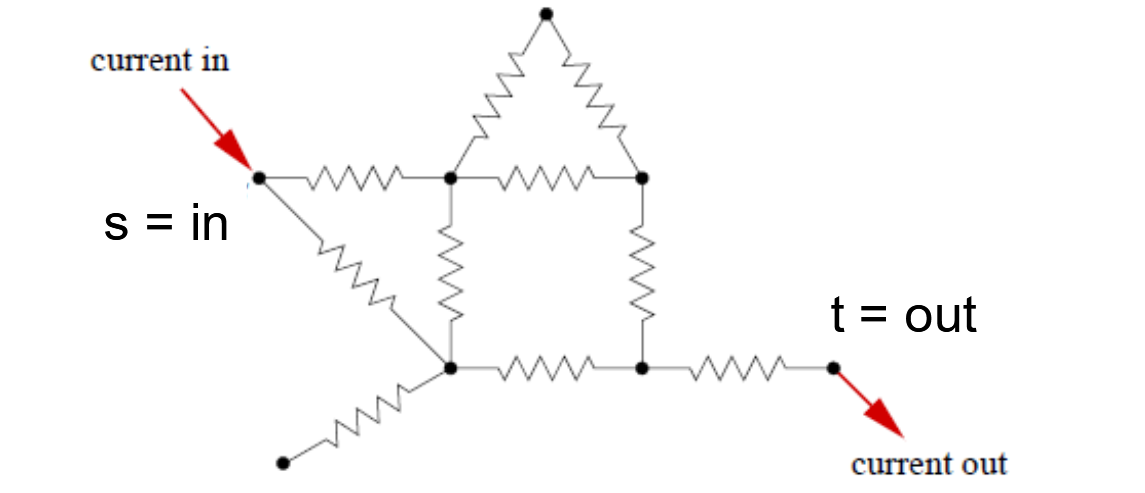
\includegraphics[width=0.9\textwidth]{img/bridge_circuit.png}
    \end{minipage}
    \hfill
    \begin{minipage}{0.35\textwidth}
        \caption{An example of a network represented as an electrical circuit, with a source node $s$ and a sink node $t$.}
        \label{fig:bridge_circuit}
    \end{minipage}
\end{figure}

Assuming unit conductances for the links (where resistance $R_{ij} = 1$, making $A_{ij} = 1/R_{ij} = G_{ij}$), the current flowing between any two connected nodes $i$ and $j$ is simply their potential difference:
\[
    i_{ij} = \frac{\Delta V_{ij}}{R_{ij}} = A_{ij}(V_i - V_j)
\]
\textit{Note:} In a weighted network, the edge weights naturally represent different conductance values (or equivalently, different inverse resistances).

By Kirchhoff's law of charge conservation, the sum of all currents entering and leaving any intermediate node must be exactly zero. The only exceptions are the source $s$ (where 1 unit enters) and the sink $t$ (where 1 unit leaves). We can write this elegantly using the Kronecker delta:
\[
    \sum_j i_{ij} = 0 \implies \sum_j A_{ij}(V_i - V_j) = \delta_{is} - \delta_{it}
\]

\subsection{Deriving the Laplacian and Solving for Potentials}

We can mathematically expand the sum of currents to reveal the graph Laplacian:
\[
    i_i = \sum_j A_{ij}(V_i - V_j) = \sum_j A_{ij}V_i - \sum_j A_{ij}V_j
\]
Because $\sum_j A_{ij} = k_i$ (the node degree), we can factor out $V_j$ using the Kronecker delta:
\[
    i_i = \sum_j (k_i \cdot \delta_{ij} - A_{ij}) \cdot V_j
\]
This term in parentheses is the exact definition of the \textbf{Combinatorial Laplacian} $L = D - A$. In vector notation, this confirms our previous derivation: $L\vec{V} = \vec{s}$, where $\vec{s}$ is the external current vector $[0, \dots, 1, \dots, -1, \dots, 0]^T$.

As established, the matrix $L$ cannot be inverted because $|L| = 0$ (its null space contains the all-ones vector $\vec{x} = (1, 1, \dots, 1)$, physically meaning that potentials are only known up to an arbitrary additive constant).

To solve the system, we apply the boundary conditions by \textbf{``grounding''} the sink node $t$, setting $V_t = 0$. We remove the $t$-th row and column from $L$ to obtain the reduced, invertible matrix $L_t$. The potentials of the remaining nodes are then strictly determined:
\[
    \vec{V}^{(st)} = L_t^{-1} \cdot \vec{s}_t
\]

\subsection{Exact Equivalence: Current Flow Centrality}

Once the potentials $V^{(st)}$ are known, we can calculate the absolute current passing through any node $i$. The absolute current through $i$ is defined as half the sum of the absolute currents on all its incident links (to avoid double counting incoming and outgoing flows):
\[
    i_i^{(st)} = \frac{1}{2} \sum_j A_{ij} |V_i^{(st)} - V_j^{(st)}|
\]

The \textbf{Current Flow Centrality (CFC)} of node $i$ is then defined as the total current passing through it, summed over all possible source-sink pairs $(s, t)$ in the network:
\[
    CFC_i = \sum_{s \neq t} i_i^{(st)}
\]

\paragraph{Connecting Random Walks and Circuits.}
The profound beauty of this network measure lies in its translation back to Random Walk probabilities. The calculated electrical potentials $V^{(st)}$ can be explicitly rewritten in terms of the network's Hitting Times ($T$), which are derived from the pseudoinverse of the Diffusive Laplacian.

By substituting the potential differences with hitting times, the current through node $i$ exactly matches the random walk passages formulation:
\[
    i_i^{(st)} = \frac{1}{2} \sum_j A_{ij} |T_{is} - T_{it} - T_{js} + T_{jt}| \quad \text{for } i \neq s, t
\]

Starting from two entirely distinct physical processes—an absorbing Markov chain and the continuous flow of current in a circuit—we arrive at the exact same topological measure of centrality. In fact, physical current flow can be fundamentally understood as a ``charged particle'' executing a random walk through the network, where the voltage differences generated by the source and ground provide a directional drift.
